\documentclass{standalone}
\usepackage{tikz}
\usepackage{ctex,siunitx}
\setCJKmainfont{Noto Serif CJK SC}
\usepackage{tkz-euclide}
\usepackage{amsmath}
\usepackage{wasysym}
\usetikzlibrary{patterns, calc}
\usetikzlibrary {decorations.pathmorphing, decorations.pathreplacing, decorations.shapes,}
\begin{document}
\small
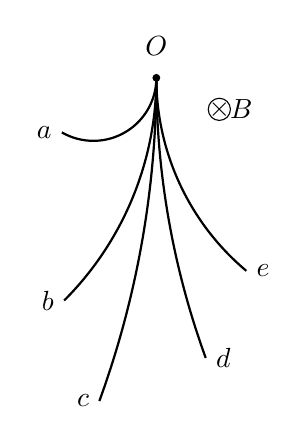
\begin{tikzpicture}[>=latex,scale=0.8]
  \draw [thick](0,0) arc (0:-120:1)node[left]{$a$};
  \draw [thick](0,0) arc (0:-45:5)node[left]{$b$};
  \draw [thick](0,0) arc (0:-20:15)node[left]{$c$};
  \draw[thick] (0,0) arc (180:200:13)node[right]{$d$};
  \draw [thick](0,0) arc (180:230:4)node[right]{$e$};
  \draw (1,-.5) [fill=white] circle (5pt);
  \node at (1,-.5){$\times$};
  \node at (1.35,-.5){$B$};
  \node at (0,.5){$O$};
  \draw (0,0) [fill=black] circle (1.5pt);
\end{tikzpicture}
\end{document}